\subsubsection{Unsichere Deserialisierung}

Der Begriff Serialisierung stammt aus der objektorientierten
Programmierung und bezeichnet die Umwandlung eines programmierten
Objekts (z. B. ein Java-, Python-Objekt) in eine Folge von Bytes.
Die Serialisierung sorgt dafür, dass erstellte Objekte nicht nur zur
Laufzeit, sondern auch danach existieren. Es ist daher eine Methode,
die für die Persistenz von Objekten verwendet wird. Sie wird auch
verwendet, um Objekte über ein Netzwerk zu übertragen (vgl. \cite{serial}).
Die Deserialisierung ist der umgekehrte Prozess der Serialisierung und
erzeugt wieder ein Objekt aus einem Bytestream.

\begin{figure}[H]
    \centering
    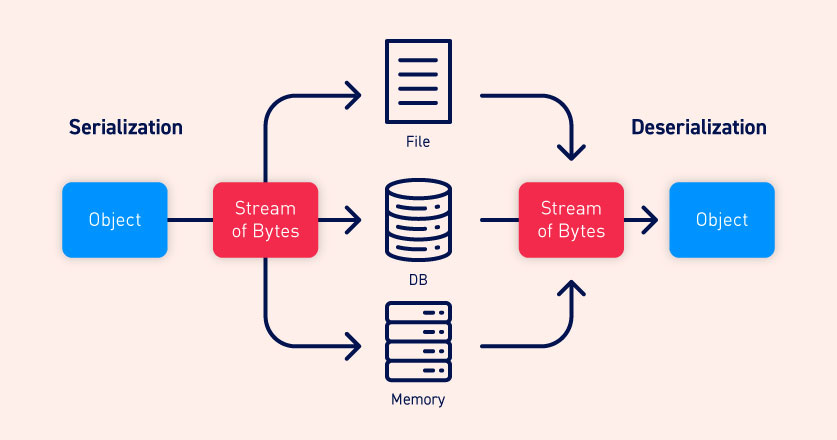
\includegraphics[scale=0.4]{images/deserialization-diagram}
    \caption{Deserialisierung Diagram (vgl. \cite{deserial-img})} \label{fig:des}
\end{figure}

Eine unsichere Deserialisierung liegt vor, wenn vom Benutzer kontrollierbare
Daten von einer Website deserialisiert werden. Dies ermöglicht es einem
Angreifer potenziell, die serialisierten Objekte zu manipulieren, um
schädliche Daten in den Anwendungscode einzuschleusen. Es ist sogar
möglich, ein serialisiertes Objekt durch ein Objekt einer völlig anderen
Klasse zu ersetzen. Alarmierenderweise werden Objekte jeder beliebigen
auf der Website verfügbaren Klasse deserialisiert und instanziiert,
unabhängig von der erwarteten Klasse. Aus diesem Grund wird die unsichere
Deserialisierung manchmal auch als "Objektinjektions"-Schwachstelle
bezeichnet  (vgl. \cite{deserial-img}).

Ein Objekt einer unerwarteten Klasse kann eine Ausnahme auslösen.
Zu diesem Zeitpunkt kann der Schaden jedoch bereits eingetreten sein.
Viele Angriffe, die auf Deserialisierung basieren, werden durchgeführt,
bevor die Deserialisierung abgeschlossen ist. Das bedeutet, dass der
Prozess der Deserialisierung selbst einen Angriff auslösen kann, auch
wenn die eigentliche Funktionalität der Website nicht direkt mit dem
bösartigen Objekt interagiert. Aus diesem Grund können auch Webseiten,
deren Logik auf stark typisierten Sprachen basiert, für diese Techniken
anfällig sein  (vgl. \cite{deserial-img}).
